\documentclass{article}
\usepackage{graphicx} % Required for inserting images
\usepackage[T1]{fontenc} % Better font encoding for accented characters
\usepackage{float}
\usepackage[spanish]{babel}
\usepackage{setspace}
\setstretch{0.9}

\title{"El mundial robado"}
\author{Omar Romero Arzate}
\date{\today}

\begin{document}


\maketitle

\section{¿Por qué el mundial de Qatar 2022 es el mundial más polémico de la historia?}

A lo largo de la gran historia de los mundiales, la gran mayoría de estos al menos han tenido un tema controversial de el cual todos hablan, alguos ejemplos puede ser la forma del balón de Sudafrica 2010, México 86 con la "mano de Dios" de armando Maradona, el mundial de 78 hablando del 6-0 de Argentina sobre Perú debido a la dictadura militar del ejercito Argentino, etc. \


Pero con todos estos ejemplos nos podemos dar cuenta de que los más famosos y polémicos tienen que ver con un país en común... ¡Argentina! muchas personas debido a su fanatismo ciego hacia Messi buscan cualquier razón para defenderlo de todo esto debido a que no fue en su tiempo, pero en 2022 paso algo muy sospechoso en Qatar... \newline

\section{Las irregularidades en la cancha}
En 2022 los inicios del mundial fueron como cualquier otro, llenos de euforia, niños comprando su albúm y llenandolo de estampas, todos buscando los jerseys de sus selecciones favoritas, pero mientras más avanzaba el torneo más se notaba el apoyo a una selección en especial... \textbf{Argentina}. \newline
Esto podria ser idea mía pero después de varios documentales acerca del mundial demuestran que mi \textit{hipotesis} es correcta, estas son algunas de las razones en las que baso mi información 

\begin{enumerate}

  \item \textbf{\textit{Récord histórico de penaltis:}}Se le concedieron 5 penaltis en 7 partidos (récord en la historia de los Mundiales). Algunos de ellos, como el choque de Livaković (Croacia) o la mano de Szczęsny (Polonia), fueron calificados de muy rigurosos.
  
  \item \textbf{\textit{Mano de Messi sin tarjeta (vs. Países Bajos): }} Lionel Messi cortó un avance neerlandés con la mano de forma deliberada. Aunque fue infracción clara, no recibió la tarjeta amarilla que correspondía.
  
  \item \textbf{\textit{Mano no sancionada de Cristian Romero (vs. Australia):}} Un remate dentro del área pegó en el brazo extendido del central argentino. La jugada no se revisó en pantalla ni se cobró penalti.
 

\end{enumerate}

A lo largo de este mundial muchos de los fanaticos de este bonito deporte nos dimos cuenta que por desgracia \textbf{"EL MUNDIAL"} esta siendo amañado por gente que solo le interesa el dinero.

\begin{figure}[H]
    \centering
    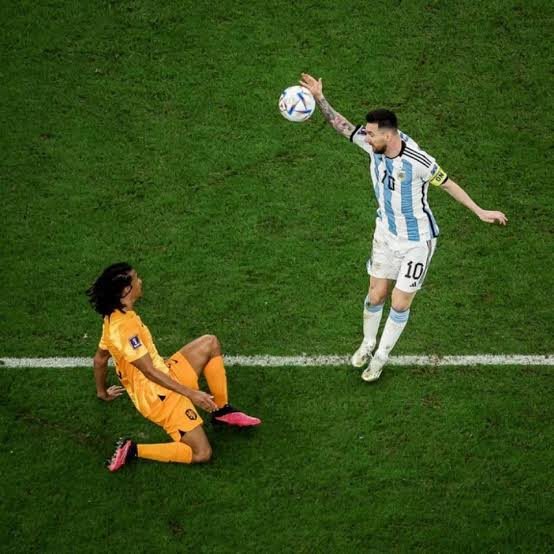
\includegraphics[width=0.5\linewidth]{Messi.jpg}
    \caption{"Mano de Messi sin repercusión alguna"}
    \label{fig:placeholder}
\end{figure}

Lastimosamente mucha gente sigue idolatrando a una persona que no ha ganado nada justamente. El ejemplo más grande de esto fue el mundial más visto por todo el mundo \textbf{\textit{"México-Cánada-Estados Unidos"}}donde de igual manera se noto el favoritismo hacia Argentina, desde la rifa de grupos, a Argentina le tocaba con Francia en un inicio y casualmente se cayó el "sistema" para que después le tocará la poderosisima "Argelia" de este mundial sobran palabras todo el mundo vio a su "Falso Campeón" morir aplastado ante España...\newline

\begin{figure}[H]
    \centering
    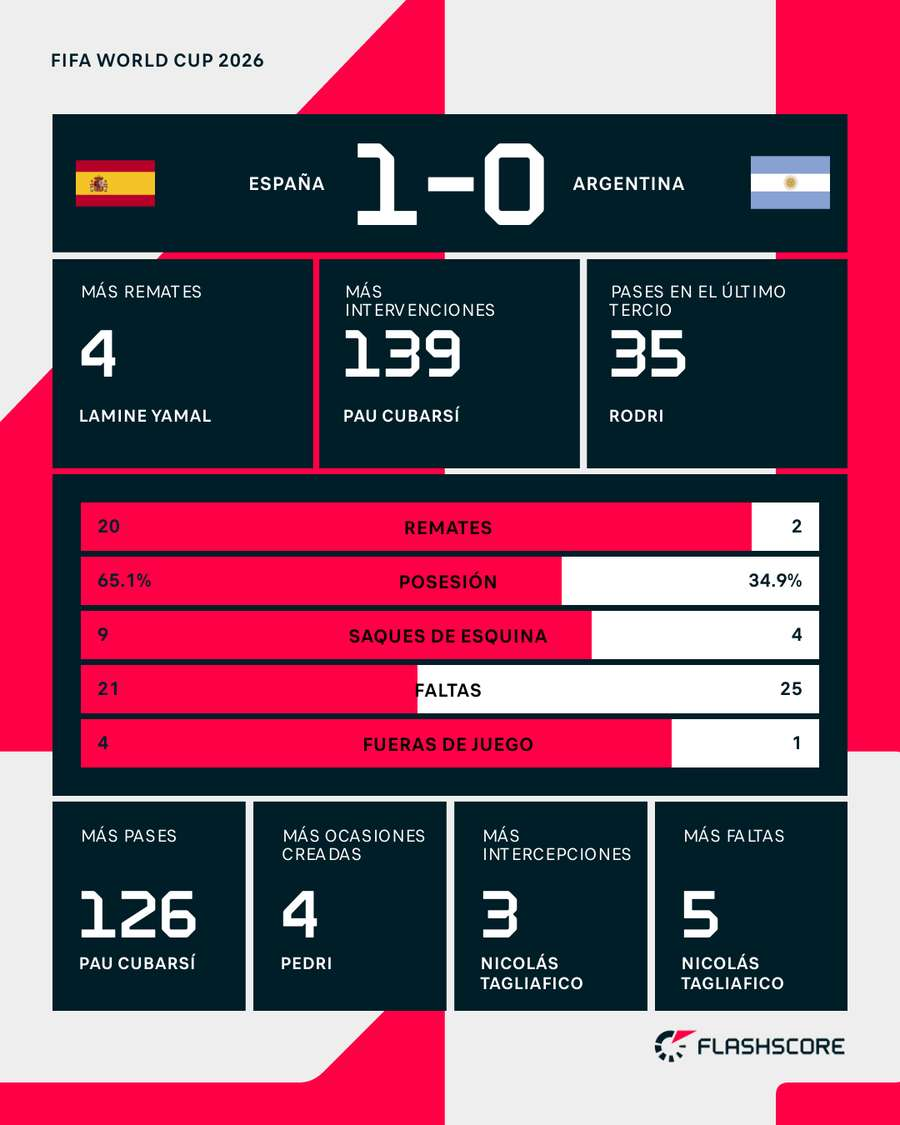
\includegraphics[width=0.40\linewidth]{EStadisticas.jpg}
    \caption{Análisis Argentina-España}
    \label{fig:placeholder}
\end{figure}


\end{document}
